\section{Reglerentwurf mit Wurzelortskurven (WOK) \buchSeite{93}}
Wurzelortskurven beschreiben die Pole linearer Systeme in Abhängigkeit von freien
Parametern.
\begin{itemize}
	\item Bei einer
	infinitesimal kleinen Änderung eines Parameters ändern die Pole auch nur infinitesimal.
	\item Wenn die n Pole eines Systems nter Ordnung für alle Parameterwerte aufgezeichnet
	werden, erscheint die Gesamtheit der Pole deshalb als n Kurven (Äste).
	\item Diese n Äste entsprechen den geometrischen Orten der Wurzeln in der komplexen
	Ebene
	\item Mithilfe der WOK kann z.B. abgeschätzt werden,
	\begin{itemize}
	\item ob es Parameterwerte gibt, die zu einem stabilen System führen,
	\item wie gross man den freien Parameter wählen/einstellen muss,
	\item welche Dämpfungen man dabei erreichen kann.
\end{itemize}
\end{itemize}


\subsection{Zeichnen der Wurzelortskurven \buchSeite{93}}
\begin{equation}
G_f(s)=\frac{KG(s)}{1+KG(s)}=\frac{K\frac{Z(s)}{N(s)}}{1+K\frac{Z(s)}{N(s)}}=\frac{KZ(s)}{\underbrace{N(s)+KZ(s)}}=\frac{Z_f(s)}{N_f(s)}
\end{equation}
\textcolor{white}{x} \hspace{9cm} charakteristisches Polynom $N_f(s)$ 

\begin{multicols}{2}
	\begin{flushleft}
		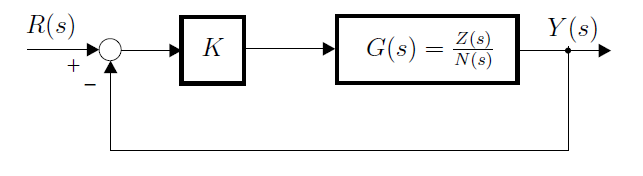
\includegraphics[width=9cm]{./images/StandardRegelkreisWOK.png}
	\end{flushleft}
\columnbreak
	\begin{flushleft}
		Beispiel: $G=\frac{1}{s-5} \quad G_f=\frac{K}{s-5+K}$ 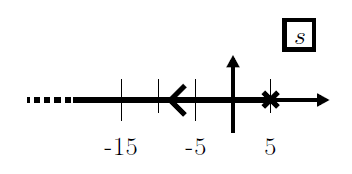
\includegraphics[width=4cm]{./images/beispielWOK.png}\\ Das charakteristische Polynom s - 5 + K zeigt eine
		Wurzel bzw. einen Pol bei s = 5 - K.
	\end{flushleft}
\end{multicols}

\subsubsection{Voraussetzungen und Vereinbarungen \buchSeite{95}}
\begin{itemize}
\item  Die UTF $G(s)=\frac{Z(s)}{N(s)}=\frac{s^m + b_{m-1}s^{m-1}+ ... + b_{1}s+b_{0}}{s^{n}+a_{n-1}s^{n-1} + ... + a_{2}s^{2}+a_{1}s + a_{0}}$
ist eine gebrochen rationale
Funktion in s mit monischen Polynomen (normierte führende Koeffizienten).
\item  In G(s) ist der Nennergrad n mindestens so gross wie der Zählergrad m; $n \geqq m$.
\item  Hat die zu untersuchende UTF eine zusätzliche Totzeit $e^{-sT_t}$ , so kann diese
z.B. mit der Padé-Approximation in die gewünschte Form gebracht werden.
\item  Hat die zu untersuchende UTF eine zusätzliche Verstärkung $k_0$, so kann diese
als Teil (d.h. als Faktor) von K betrachtet werden.
\item  Die WOK werden gezeichnet bezogen auf positive Verstärkungen K. Zu beachten
ist, dass K eine allfällig vorhandene Verstärkung k0 beinhaltet.
\end{itemize}

\subsubsection{Grundsätzliches Aussehen der WOK \buchSeite{96}}
\begin{minipage}{14cm}
	\begin{itemize}
		\item  Das charakteristische Polynom $N_f (s) = N(s)+K \cdot Z(s)$ hat für jeden K-Wert
		n Wurzeln. Visualisiert man die Wurzeln für alle positiven K-Werte, dann
		ergeben sich n kontinuierliche Linien (Äste).
		\item  Da Pole immer reell oder (paarweise) komplex-konjugiert sind, ist das Gesamtbild
		der WOK immer symmetrisch bezüglich der reellen Achse.
	\end{itemize}
\end{minipage}
\hspace{0.5cm}
\begin{minipage}{4cm}
	\textbf{Merke:} \\
		m = Anz. Nullstellen \& \\
		n = Anz. Pole von $G_0$
\end{minipage}
\begin{itemize}
		\item  Für K = 0 sind die n Wurzeln von $N_f(s)$ und N(s) identisch und entsprechen
		den n Polen von G(s).
		Für $K \rightarrow \infty$ streben m der Wurzeln von $N_f(s)$ zu den Wurzeln von Z(s). Die
		restlichen n-mWurzeln von Nf (s) streben entlang von Geraden asymptotisch
		ins ‘Unendliche’.
		Damit teilen sich die n Äste auf in zwei Arten:
		\begin{enumerate}
			\item m Äste, die von m Polen von G(s) zu den m Nullstellen von G(s) gehen
			\item n - m Äste, die von n - m Polen von G(s) ins Unendliche laufen.
		\end{enumerate}
\end{itemize}


\subsubsection{Regeln zum Zeichnen der WOK \buchSeite{96}}
\begin{enumerate}
\item \textbf{Pol-/Nullstellen-Plan:}\\
Die Pole $p_k (k = 1...n)$ von G(s) werden als x in der komplexen Ebene eingezeichnet;
dies sind die Startpunkte aller n Äste. Die Nullstellen $z_k (k = 1...m)$
werden als o eingezeichnet; dies sind die Endpunkte von m Ästen.
\item \textbf{Reelle Achse:}\\
Diejenigen Punkte der reellen Achse welche zu den WOK gehören, haben rechts
von sich auf der reellen Achse eine ungerade Anzahl von Polen und Nullstellen.
Um diese Punkte einzuzeichnen, kann man von ‘genug weit’ rechts startend
der reellen Achse entlang ‘genug weit’ nach links fahren. Dabei wechselt der
Zeichenstift bei jedem Pol und bei jeder Nullstelle den Status zwischen ‘nicht
zeichnend’ bzw. ‘zeichnend’. Der Anfangsstatus ist ‘nicht zeichnend’.
\begin{figure}[h!]
	\begin{center}
		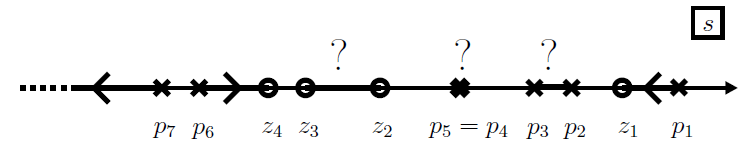
\includegraphics[width=12cm]{./images/reelleAchsePoleNullWOK.png}
	\end{center}
	\caption{Zur WOK gehörende Teile der reellen Achse}
	\label{beispielAchse}
\end{figure}

Im etwas komplexeren Beispiel von Abb.\ref{beispielAchse} entstehen 6 Striche. Einer davon
ist nur ein Punkt: beim Doppelpol $p_4 = p_5$. Einer der Striche verschwindet
gegen links im Unendlichen. Zwei Striche verbinden Pol mit Nullstelle; dies
sind gültige WOK-Äste. An den mit ? versehenen Stellen ist offensichtlich die
Situation noch unbefriedigend.


\item \textbf{Asymptoten: Schnittpunkt und Richtungen:}\\
Wenn $n > m$ gilt, dann streben n-m Äste der WOK asymptotisch gegen
Unendlich. Die n-m Asymptoten sind Geraden. Sie schneiden sich im Punkt
\begin{multicols}{2}
		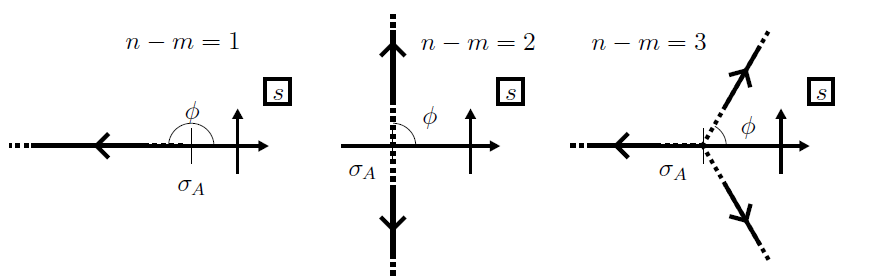
\includegraphics[width=10cm]{./images/asymptotenrichtunge.png}
Abbildung \ref{Asymptotenrichtungen}: Asymptotenrichtungen bei WOK für die Fälle n - m = 1, 2, 3 (Weitere im Anhang)
		\label{Asymptotenrichtungen}
\columnbreak
	\begin{flushright}
		\[\boxed{\sigma_A=\frac{\sum\limits_{k=1}^{n} Re(p_k)-\sum\limits_{k=1}^{m} Re(z_k)}{n-m}}\]
	\end{flushright}
\end{multicols}
Eine der Asymptoten zeigt in die Richtung $\phi = \frac{\pi}{n-m}$. Die weiteren Asymptoten
sind dann gleichmässig um den Winkel $\frac{2\pi}{n-m}$ versetzt,

\begin{multicols}{2}
\item \textbf{Verzweigungspunkte, Vereinigungspunkte:}\\
Erklärung zu den In Abb. \ref{Asymptotenrichtungen} mit ? versehenen Stellen. Treffen
zwei Äste, von Polen her kommend, aufeinander, dann verzweigt
sich die WOK. Beim Verzweigungspunkt treten die Äste (meistens) rechtwinklig
aus der reellen Achse aus. Entsprechend können auch zwei Äste im rechten
Winkel auf die reelle Achse zustreben und nach dem Vereinigungspunkt auf
dieser weiterlaufen. In Abb. \ref{KomplettWOK} ist die Skizze der WOK aus Abb. \ref{beispielAchse}
komplettiert: $\sigma_{V,1}$ ist dabei ein Vereinigungspunkt, $\sigma_{V,2}$ und $\sigma_{V,3}$ sind zwei
Verzweigungspunkte. $\sigma_{V,1}$ und $\sigma_{V,2}$ sind näherungsweise mit zwei Kreisbögen
verbunden. \\

\columnbreak
Da n-m = 3 gilt, entstehen drei Asymptoten, deren Schnittpunkt
bei $\sigma_A$ liegt.

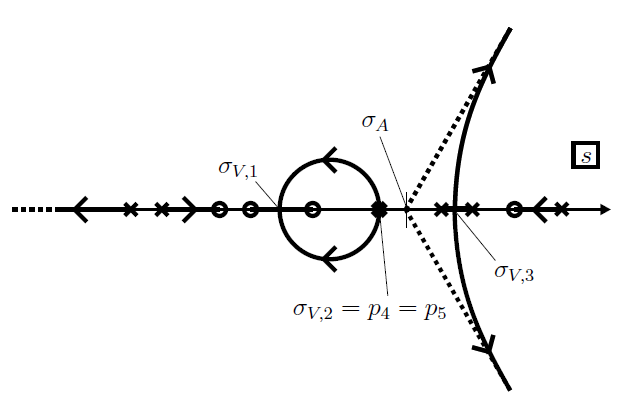
\includegraphics[width=6.5cm]{./images/KomplettWOK.png}\\
Abbildung: \ref{KomplettWOK} {Komplettierte Skizze der WOK Abb: \ref{Asymptotenrichtungen}} \label{KomplettWOK}
\end{multicols}
Für eine \textbf{einfache Skizze} genügt es meistens, die Verzweigungs- bzw. Vereinigungspunkte ‘etwa in der Mitte’ zwischen den involvierten zwei Polen bzw. Nullstellen zu plazieren.
\end{enumerate}

\subsection{Interpretation der Wurzelortskurven \buchSeite{100}}

\subsubsection{Auslegen eines P-Reglers mithilfe der WOK \buchSeite{101}}
\begin{figure}[h!]
	\begin{subfigure}[t]{8.5cm}
Beispiel: Eine Strecke \[G_s(s)=\frac{5}{s^2 + 6s +8}=\frac{5}{(s+2)(s+4)}\] soll mit einem P-Regler mit
 möglichst grosser Verstärkung $K_R$ geregelt werden, wobei alle Pole eine minimale
 Dämpfung $\xi = 0.7$ haben sollen.\\


	\end{subfigure}$\qquad$
	\begin{subfigure}[t]{10cm}
		Lösung:
		 \[G_0=K_R\cdot\underbrace{\frac{5}{(s+2)(s+4)}}_{G_s(s)}=\underbrace{K_r\cdot 5}_{K} \cdot\underbrace{\frac{1}{(s+2)(s+4)}}_{G(s)}\]
		%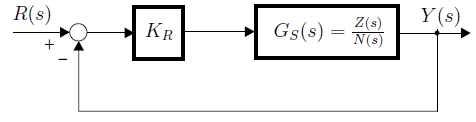
\includegraphics[width=7cm]{./images/PReglerBeispielWOK1.png}
	\end{subfigure}
\end{figure}

Zusammenfassung des Vorgehens:\\
\begin{center}
    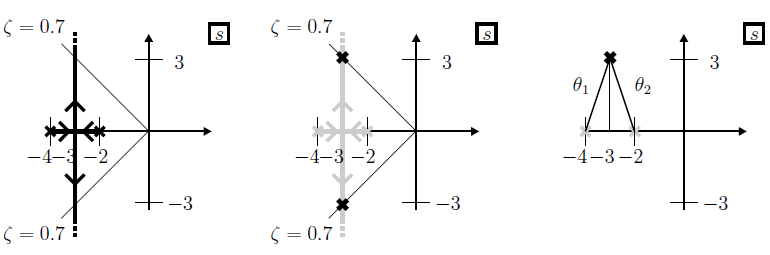
\includegraphics[width=12cm]{./images/PReglerBeispielWOK2.png}
\end{center}

\begin{multicols}{2}
    \begin{itemize}
    	\item  \textbf{Links:} Die WOK-Äste treffen sich bei -3 und laufen vertikal weiter.
    	\item  \textbf{Mitte:} Die Dämpfung nimmt mit steigendem Wert von K (bzw. $K_R$) ab; die
    	Pole kommen auf die Schnittpunkte der WOK mit den Winkelhalbierenden um eine Dämpfung von $\xi$ = 0.7 zu erreichen.
    	\item  \textbf{Rechts:} Um den Wert K (bzw. $K_R$) zu bestimmen, muss einer der platzierten	Pole betrachtet werden. Der Wert von K berechnet sich aus den Abständen $\theta_i$ dieses Pols zu den Polen von G(s) und den Abständen $\lambda_i$ dieses Pols zu den
    	Nullstellen von G(s): 
        \[
            K=\frac{\prod_{i=1}^{n} \theta_i}{\prod_{i=1}^{m}\lambda_i}=\frac{\theta_1\theta_2\cdots\theta_n}{\lambda_1\lambda_2\cdots\lambda_m} \\
        \]
        Im konkreten Beispiel hat es keine Nullstellen, womit das entsprechende Produkt
    	gleich Eins wird. 	Damit ist $K=\theta_1\theta_2$ .Mit $\theta_1=\theta_2=\sqrt{3^2+1^2}$ ergibt sich \textbf{K = 10} bzw. $K_R = K/5 = 2$.
    \end{itemize}
\end{multicols}


\subsubsection{Auslegen dynamischer Regler mithilfe der WOK \buchSeite{102}}


\subsubsection{Allgemeine Stabilitätsanalyse mithilfe der WOK \buchSeite{109}}
Der Regelkreis $K\cdot G_s(S)=K\cdot\frac{1}{S^2+\alpha s + 2}$ mit den zwei Parametern K und $\alpha$ hat das charakteristische
Polynom $N_f(s)=N(s) + K\cdot Z(s) = s2 + \alpha s + (2 + K)$. Denkt man sich jeweils einen der
Parameter als fix gegeben, kann mithilfe der WOK den Einfluss des anderen Parameters
auf die Pollage des geschlossenen Regelkreises untersucht werden:

Fall 1, $\alpha$ fix, K variabel
Dies entspricht dem bisher besprochenen Vorgehen, bei dem die Kreisverstärkung
K untersucht wird, und bei dem die Summe Nf (s) so interpretiert wird:
$N_f(s)=\underbrace{s^2+\alpha s + 2} +\underbrace{K}\cdot\underbrace{1} $\\
\textcolor{white}{x} \hspace{12.25cm} $P_N(s)=N(s) \quad Faktor  \quad P_z(s)=Z(s)$
Fall 2, $\alpha$ variabel, K fix Bei einer Untersuchung bezüglich $\alpha$ ist dagegen
$N_f(s)=\underbrace{s^2+ 2 + K} +\underbrace{\alpha}\cdot\underbrace{s} $\\
\textcolor{white}{x} \hspace{13.5cm} $P_N(s) \qquad Faktor  \quad P_z(s)$
